%
% $RCSfile: branching.tex,v $
%
% Copyright (C) 2002-2008. Christian Heller.
%
% Permission is granted to copy, distribute and/or modify this document
% under the terms of the GNU Free Documentation License, Version 1.1 or
% any later version published by the Free Software Foundation; with no
% Invariant Sections, with no Front-Cover Texts and with no Back-Cover
% Texts. A copy of the license is included in the section entitled
% "GNU Free Documentation License".
%
% http://www.cybop.net
% - Cybernetics Oriented Programming -
%
% http://www.resmedicinae.org
% - Information in Medicine -
%
% Version: $Revision: 1.1 $ $Date: 2008-08-19 20:41:05 $ $Author: christian $
% Authors: Christian Heller <christian.heller@tuxtax.de>
%

\subsubsection{Branching}
\label{branching_heading}
\index{Branching}
\index{Branch}
\index{Conditional Branching}
\index{Unconditional Branching}
\index{Goto (Jump) Command}
\index{Condition}
\index{Alternative}
\index{Choice}
\index{Multiple Condition}
\index{Switch}
\index{Case}

A block of statements that get only executed at special occasions is called a
\emph{Branch}. Two kinds of branching exist: \emph{Conditional Branching} and
\emph{Unconditional Branching}. An implementation of the latter is the well-known
but also disliked \emph{goto} (\emph{jump}) command. The former depends on a
\emph{Condition}, also called \emph{Alternative} or \emph{Choice} (figure
\ref{condition_figure}), that is its statements are only executed if the
condition's result is true. That way, a condition can change the flow of a
program. A code example follows; it shows conditional branching:

\begin{scriptsize}
    \begin{verbatim}
    if (condition) {
        statements;
    } else {
        statements;
    }
    \end{verbatim}
\end{scriptsize}

\begin{figure}[ht]
    \begin{center}
        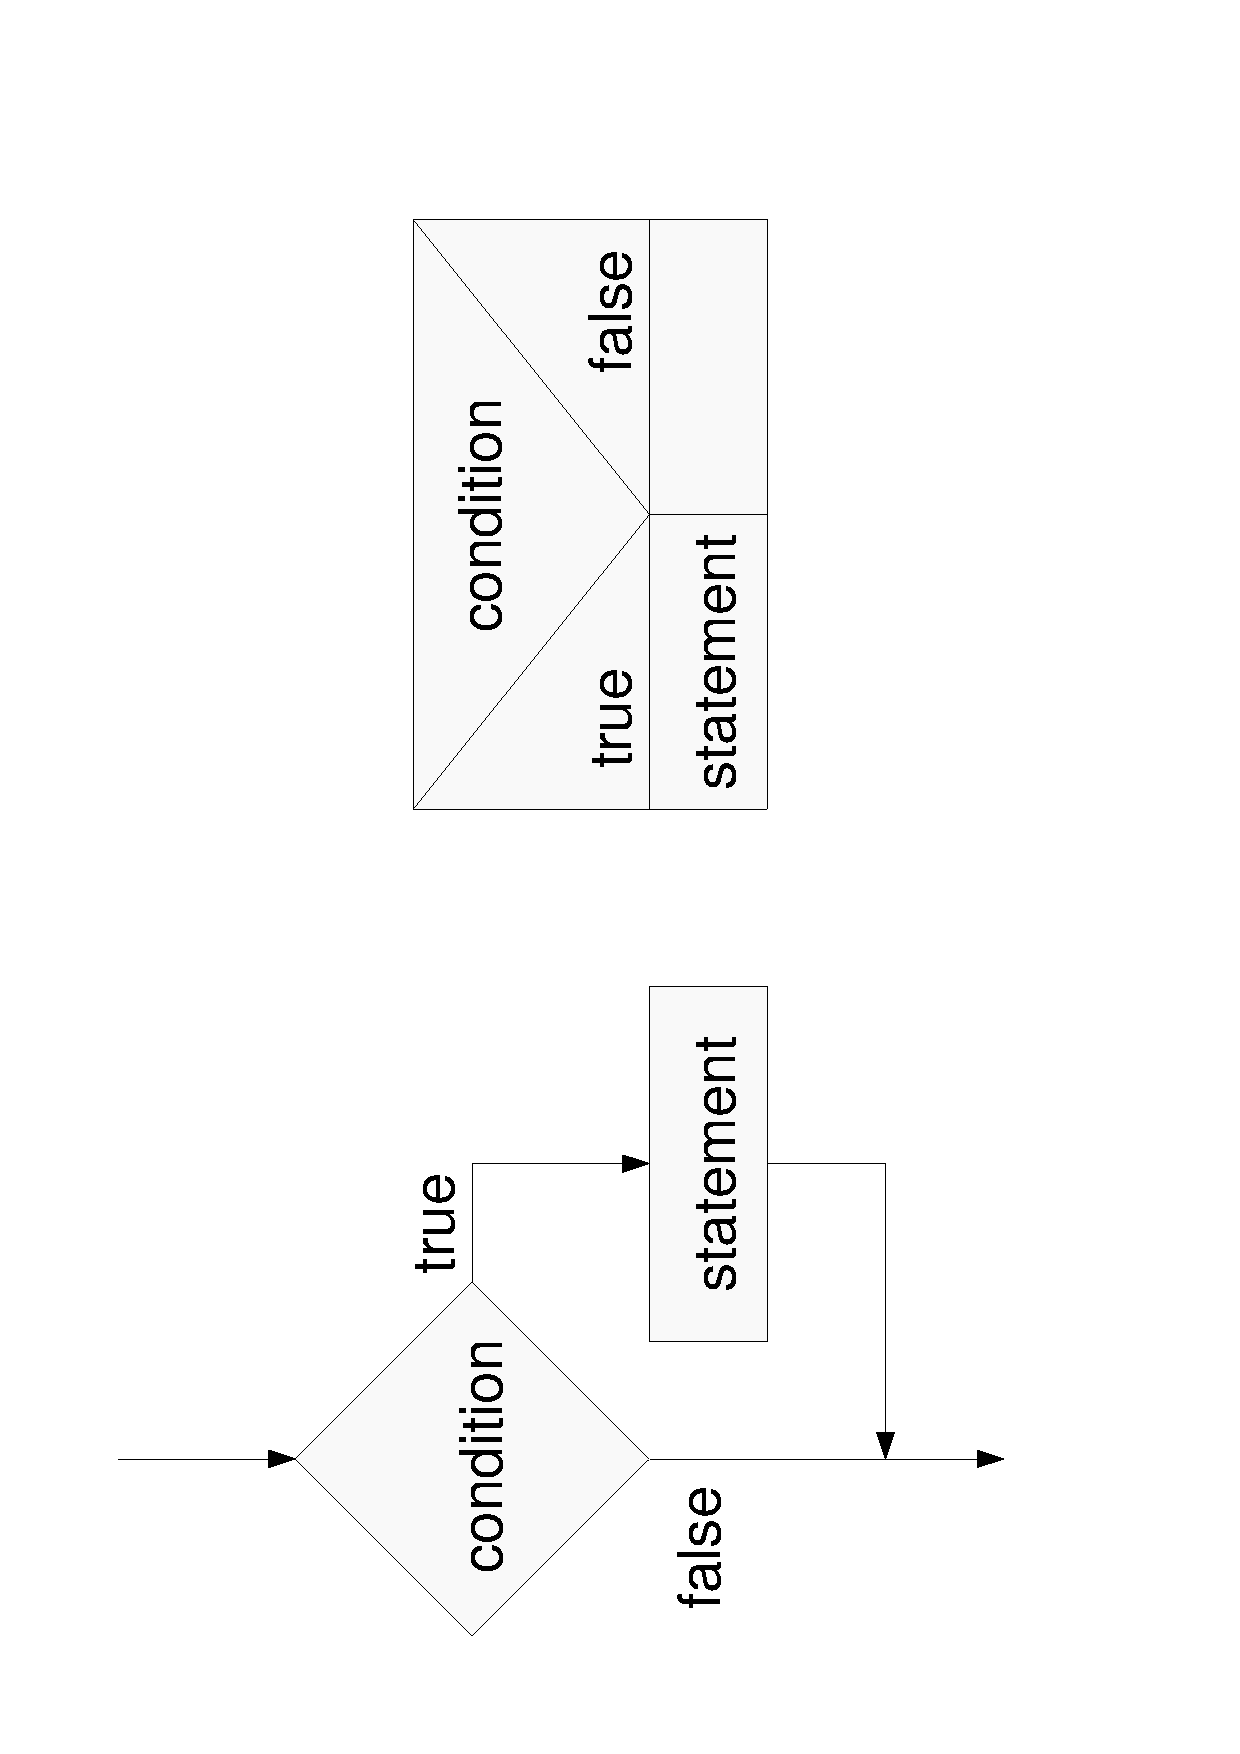
\includegraphics[scale=0.3,angle=-90]{graphic/condition.pdf}
        \caption{Condition as Program Flow Chart and Structure Chart}
        \label{condition_figure}
    \end{center}
\end{figure}

Many programming languages offer a \emph{Multiple Condition} control structure
like \emph{switch} or \emph{case}. It is a comfortable possibility to let a
program make a choice out of many alternatives:

\begin{scriptsize}
    \begin{verbatim}
    switch (condition) {
        case constant1:
            statements;
        case constant2:
            statements;
        default:
            statements;
    }
    \end{verbatim}
\end{scriptsize}

Essentially, however, it is a subsumption of a number of simple conditions which
are mostly called \emph{if-else}, and therefore replaceable by such, as shown
following:

\begin{scriptsize}
    \begin{verbatim}
    if (condition == constant1) {
        statements;
    } else if (condition == constant2) {
        statements;
    } else {
        statements;
    }
    \end{verbatim}
\end{scriptsize}

The multiple condition is conceptually no innovation in comparison with the
simple condition and hence pure convenience for the programmer. The interpreter
described in chapter \ref{cybernetics_oriented_interpreter_heading} uses solely
if-then statements.
